\chapter{Control Theoretic Model and Problem Statement}\label{c:control}

The following chapter explains the 

\section{Basics of Control Theory}\label{c:control:s:basics}

A general nonlinear, dynamical system $\Sigma$ can be described \cite{Adamy2014}

\begin{align}
\begin{split}
\ve{\dot{x}} &= \ve{f}\left(\ve{x},\ve{u}, t\right) \\
\ve{y} &= \ve{h}\left(\ve{x},\ve{u},t \right)
\end{split}
\label{c:control:e:nonlinearsystem}
\end{align}
\nomenclature{$\ve{x}$}{State Vector of a Dynamical System}
\nomenclature{$\ve{u}$}{Input Vector of a Dynamical System}
\nomenclature{$\ve{y}$}{Output Vector of a Dynamical System}
\nomenclature{$\ve{f}$}{Vector Function of a Nonlinear Dynamical System}
\nomenclature{$\ve{h}$}{Output Vector Function of a Nonlinear Dynamical System}


Where $t \in \mathbb{R}^+$ is the time, $\ve{x} \in \mathbb{R}^{n_x}$ is called the state vector, or states, and $\ve{u} \in \mathbb{R}^{n_u}$ the input vector, or inputs, of the system. The output $\ve{y} \in \mathbb{R}^{n_y}$ of the system is described by the functions$\ve{h}~:\mathbb{R}^{n_x},\mathbb{R}^{n_u},\mathbb{R}^+ \mapsto \mathbb{R}^{n_y}$ and the evolution of the system over time is given by $\ve{f}:~\mathbb{R}^{n_x},\mathbb{R}^{n_u},\mathbb{R}^+ \mapsto \mathbb{R}^{n_x} $.\\

The System given by Eq. \ref{c:control:e:nonlinearsystem} can be used to describe almost every natural or technical system.\newline
Due to several reasons, e.g. controller design, measurements, modelling issues and errors, most technical applications simplify the model by assuming linear, time invariant (LTI) behaviour. The LTI system is represented by a set of first-order differential equations \cite{Lunze2014} called state space representation:

\begin{align}
\begin{split}
\ve{\dot{x}} &= \ma{A}~\ve{x} + \ma{B}~\ve{u} \\
\ve{y} &= \ma{C}~\ve{x} + \ma{D}~\ve{u}
\end{split}
\label{c:control:e:ltisystem}
\end{align}
\nomenclature{$\ma{A}$}{State Matrix of a Dynamical System}
\nomenclature{$\ma{B}$}{Input Matrix of a Dynamical System}
\nomenclature{$\ma{C}$}{Output Matrix of a Dynamical System}
\nomenclature{$\ma{D}$}{Feedthrough Matrix of a Dynamical System}
The state matrix $\ma{A} \in \mathbb{R}^{n_x\times n_x}$ describes the influence of the current states, the input matrix $\ma{B} \in \mathbb{R}^{n_x\times n_u}$ the influence of the current input on the future states and output. The output is given by the output matrix $\ma{C} \in \mathbb{R}^{n_y\times n_x}$ and the feedthrough matrix $\ma{D} \in \mathbb{R}^{n_y\times n_u}$.\\

Both Eq. \ref{c:control:e:nonlinearsystem} and Eq. \ref{c:control:e:ltisystem} are able to generate a variety of different controllers, see e.g. \cite{Adamy2014},\cite{Lunze2014}, \cite{Lunze2016}. The ability to design controller via state space methods is connected to a high information content about (physical) parameters and equations or in form of measurement data.\\

Hence a more compressed form is commonly used to design controller for most technical and industrial applications. The transfer function matrix \cite[p.20]{Lunze2014} $\ma{G} \in \mathbb{C}^{n_y\times n_u}$ can be derived via the Laplacetransform of Eq.\ref{c:control:e:ltisystem}:

\begin{align}
\begin{split}
\ma{G} &= \ma{C} \left(s \ma{I} - \ma{A} \right)^{-1} \ma{B} + \ma{D} \\
\end{split}
\label{c:control:e:TransferFunctionMatrix}
\end{align}
\nomenclature{$\ma{G}$}{Transfer Function Matrix}

The transfer function matrix consist of single transfer functions $g_{ij}(s)~, i \leq n_y, j \leq n_u$ and maps the transformed input of a system directly to its  transformed output. It describes the relationship between input and output directly and is hence a compact form of describing the behaviour of LTI systems. To control a system with two outputs in every wanted direction a necessary condition is given by $n_y \leq n_u$. It is assumed that all following systems suffice $\dim{\ma{G}} = n_y \times n_y$.  \\

\section{Feedback Control in Presence of Uncertain Signals}

The aim of control theory is to manipulate a systems trajectory via its inputs in such a way, that a desired output is reached and maintained. To do this, several techniques can be used. Most commonly the systems desired output, the setpoint $\ve{y}_r$, is compared to the actual output of the system $\ve{y}$ via a feedback loop. The result of this comparison is called the error $\ve{e} \in \mathbb{R}^{n_y}$ \nomenclature{$\ve{e}$}{Error Signal of a Feedback Loop}. This signal is fed into the controller $\ma{K} \in \mathbb{C}^{n_y \times n_y}$ \nomenclature{$\ma{K}$}{Controller of a Dynamical System} and the result is used as an input for the system. This approach is called feedback control, see e.g. \cite{Astrom2009}, with a single degree of freedom controller.\\

A variation of this approach is to use a weighted set point and output signal to generate the input. The pair of weighting matrices $\ma{K}_r$  for the setpoint and $\ma{K}_y$ for the output is called a two degree of freedom controller. The structure of such a controller design is shown in Fig. \ref{c:control:f:2dofclosedloop}.

\begin{figure}[H]
\begin{minipage}[b]{\textwidth}
\centering
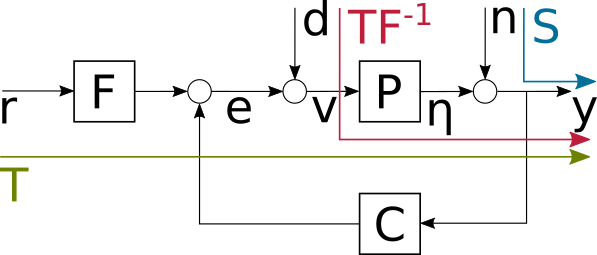
\includegraphics[width=0.9\textwidth]{./Graphics/2DOFCLOSEDLOOP.png}
\caption{Two Degree of Freedom Feedback Control}
\label{c:control:f:2dofclosedloop}
\end{minipage}
\end{figure}

In Fig. \ref{c:control:f:2dofclosedloop} other signals are added as well.The disturbances $\ve{d} \in \mathbb{R}^{n_y}$ are acting on the weighted error. The signal $\ve{v} \in \mathbb{R}^{n_y}$ is the disturbed input of the plant. $\ve{\eta} \in \mathbb{R}^{n_y}$ is the plants output without measurement noise which will be referred to as real output. The measurement noise is given by $\ve{n} \in \mathbb{R}^{n_y}$. The superposition of noise and real output is $\ve{y}$ which will be referred to simply as output. The closed loop transfer function is given by:

\begin{align}
\begin{split}
\ve{y} &= \left[\ma{I} - \ma{G} \ma{K}_y\right]^{-1} \left[ \ma{G}\ma{K}_r \ve{y}_r + \ve{n} + \ma{G} \ve{d} \right]
\end{split}
\label{c:control:e:2dofclosedloop}
\end{align}
\nomenclature{$\ve{d}$}{Disturbance Vector of a Dynamical System}
\nomenclature{$\ve{n}$}{Measurement Noise Vector of a Dynamical System}

Eq. \ref{c:control:e:2dofclosedloop} relates the output of a system to the influences of set point, disturbances and measurement noise. 
Rewriting the equation as:

\begin{align}
\begin{split}
\ve{y} &= \ma{T}\ve{y}_r + \ma{S} \left[ \ve{n} + \ma{G} \ve{d} \right]
\end{split}
\label{c:control:e:sensitivityclosedloop}
\end{align}
defines the Sensitivity Function $\ma{S} = \left[ \ma{I} - \ma{G} \ma{K}_y\right]^{-1} \in \mathbb{C}^{n_y \times n_y}$ which relates the influences of measurement noise and load disturbance to the systems outputs. The Complementary Sensitivity Function $\ma{T} = \left[\ma{I} - \ma{G} \ma{K}_y\right]^{-1} \ma{G} \ma{K_r} \in \mathbb{C}^{n_y \times n_y}$ describes the response to the reference signal.Both Functions play an important role in the investigation of the systems Robustness and are connected to each other via $\ma{T} = \ma{S} \ma{G} \ma{K}_r$.\\

\section{Robustness and Stability of Feedback Control Systems}

Robustness refers in general to the stability of the system in presence of uncertainties and has been studied extensively, see e.g. \cite{Zhou1998},\cite{Zhou1996}, \cite{DoyleFeedbackTheory}.
To give a better understanding of the relevant points of the subject both SISO and MIMO cases are presented. \\

For any given SISO system with a transfer function $g : \mathbb{R} \mapsto \mathbb{C}$ we see from Eq. \ref{c:control:e:2dofclosedloop} that the behaviour of the output with respect to measurement noise and disturbances is strongly dependent on the sensitivity function. A necessary condition for the system to reach the reference is that disturbance and noise are attenuated  near the steady state. Furthermore the destabilizing effect due to uncertain signals can be quantified via the maximum of the sensitivity function. Therefore the Maximum Sensitivity is defined as:

\begin{align}
\begin{split}
M_S & = \max_\omega \left| S \right| \\
& \geq \left| \frac{1}{1 - g~k_y}\right|
\end{split}
\label{c:control:e:maxsensitivity}
\end{align}

With Eq. \ref{c:control:e:maxsensitivity} an upper boundary on the gain can be found and be used as a measure of robustness of the closed loop \cite[p.323 ff.]{Astrom2009}. The maximum sensitivity is also connected to the nyquist stability and the stability margin of a system via:

\begin{align}
\begin{split}
M_S &= \frac{1}{s_M} \\
&= \frac{1}{1 - \max_\omega \left| g ~k_y \right|}
\end{split}
\label{c:control:e:maxsensitivitynyquist}
\end{align}

Or rearranged to be:

\begin{align}
\begin{split}
\max_\omega \left| g~k_y\right| &= 1 - s_M
\end{split}
\end{align}

Due to Eq. \ref{c:control:e:maxsensitivitynyquist} the maximum gain of the open loop is limited by the maximum sensitivity. Hence, the critical point is only encircled iff the maximum sensitivity is zero. Hence the system is only stable in the sense of the Nyquist Criterion if the maximum sensitivity is sufficiently small.\\

\begin{figure}[H]
\begin{minipage}[b]{\textwidth}
\centering
\input{./Graphics/MS.pdf_tex}
\caption{Maximum Sensitivity}
\label{c:control:f:MaximumSensitivity}
\end{minipage}
\end{figure}


While the maximum sensitivity is well definied for SISO systems, a MIMO system requires a more general approach due to the interconnection of the systems out- and inputs. A general condition is given by the Small Gain Theorem \cite[p.150 ff.]{Skogestad2005MultivariableDesign}. The theorem states, that a given feedback system is stable iff the open loop transfer function matrix is stable and its sufficient conditioned matrix norm is less than 1 over all frequencies.

\begin{align}
\lVert \ma{G} \ma{K}_y \rVert < 1 ~\forall \omega
\label{c:control:e:SmallGainTheorem}
\end{align}

Eq. \ref{c:control:e:SmallGainTheorem} can be used with several matrix norms and can be viewed as an MIMO Interpretation of the Nyquist Criterion. \\

For further robustness analysis, the concept of singular values has to be investigated. The singular value decomposition, see e.g. \cite[p.144 f.]{2013Springer-HandbuchIII},states that any matrix $\ma{G} \in \mathbb{C}^{n_a\times n_b}$ can be factorized such that

\begin{align}
\ma{G} &= \ma{U}\ma{\sigma}\ma{V}^*
\label{c:control:e:SVD}
\end{align}

Where as $\ma{U} \in \mathbb{C}^{n_a \times n_a}$ and $\ma{V} \in \mathbb{C}^{n_b \times n_b} $ are unitary matrices representing the left and right eigenvectors of matrix. The matrix $\ma{\sigma} \in \mathbb{C}^{n_a \times n_b}$ is a rectangular, diagonal matrix consisting of the singular values $\sigma \in \mathbb{C}$ of $\ma{G}$. A practical point of view suggest a rotation of any given input vector via $\ma{V}^*$, distributing the magnitude of the input over the columns of $\ma{\sigma}$, where they are scaled according to the magnitude of the corresponding singular value. Then the scaled and rotated vector is once again rotated by $\ma{U}$ and distributed over the output vector. \\

\begin{figure}[H]
\begin{minipage}[b]{\textwidth}
\centering
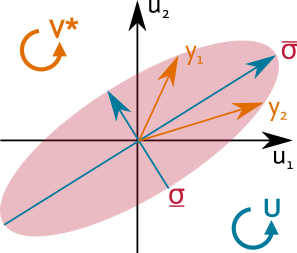
\includegraphics[scale=1]{./Graphics/SVD.png}
\caption{Graphical Interpretation of the Singular Value Decomposition}
\label{c:control:f:SVD}
\end{minipage}
\end{figure}



An example of this process is illustrated in Fig. \ref{c:control:f:SVD} for a system with two inputs $u_1,u_2$ and two outputs $y_1,y_2$. The output is bounded by the ellipsoid described by the maximum singular value $\overline{\sigma}$ and the minimum singular value $\underline{\sigma}$. The orientation and the magnitude of the outputs change depending on the frequency but will never exceed these limits. The singular values of a matrix are hence representing the highest possible gain for any given input if $\ma{U} = \ma{V}^* = \ma{I}$. With that, the induced 2-Norm for a matrix can be defined as:

\begin{align}
\begin{split}
\lVert \ma{G} \rVert_2 &= \frac{\lVert \ma{G}\ma{u}\rVert_2}{\lVert \ma{u} \rVert_2} \\
&= \max \sqrt{\lambda\left( \ma{G}^* \ma{G}\right)} \\
&= \overline{\sigma}
\end{split}
\label{c:control:e:MaxSingularValue}
\end{align}

\section{Gain Scheduling} % (fold)
\label{c:control:s:gainsched}

% section gain_scheduling (entrol:s:gainschednd)